
%% bare_jrnl.tex
%% V1.3
%% 2007/01/11
%% by Michael Shell
%% see http://www.michaelshell.org/
%% for current contact information.
%%
%% This is a skeleton file demonstrating the use of IEEEtran.cls
%% (requires IEEEtran.cls version 1.7 or later) with an IEEE journal paper.
%%
%% Support sites:
%% http://www.michaelshell.org/tex/ieeetran/
%% http://www.ctan.org/tex-archive/macros/latex/contrib/IEEEtran/
%% and
%% http://www.ieee.org/



% *** Authors should verify (and, if needed, correct) their LaTeX system  ***
% *** with the testflow diagnostic prior to trusting their LaTeX platform ***
% *** with production work. IEEE's font choices can trigger bugs that do  ***
% *** not appear when using other class files.                            ***
% The testflow support page is at:
% http://www.michaelshell.org/tex/testflow/


%%*************************************************************************
%% Legal Notice:
%% This code is offered as-is without any warranty either expressed or
%% implied; without even the implied warranty of MERCHANTABILITY or
%% FITNESS FOR A PARTICULAR PURPOSE! 
%% User assumes all risk.
%% In no event shall IEEE or any contributor to this code be liable for
%% any damages or losses, including, but not limited to, incidental,
%% consequential, or any other damages, resulting from the use or misuse
%% of any information contained here.
%%
%% All comments are the opinions of their respective authors and are not
%% necessarily endorsed by the IEEE.
%%
%% This work is distributed under the LaTeX Project Public License (LPPL)
%% ( http://www.latex-project.org/ ) version 1.3, and may be freely used,
%% distributed and modified. A copy of the LPPL, version 1.3, is included
%% in the base LaTeX documentation of all distributions of LaTeX released
%% 2003/12/01 or later.
%% Retain all contribution notices and credits.
%% ** Modified files should be clearly indicated as such, including  **
%% ** renaming them and changing author support contact information. **
%%
%% File list of work: IEEEtran.cls, IEEEtran_HOWTO.pdf, bare_adv.tex,
%%                    bare_conf.tex, bare_jrnl.tex, bare_jrnl_compsoc.tex
%%*************************************************************************

% Note that the a4paper option is mainly intended so that authors in
% countries using A4 can easily print to A4 and see how their papers will
% look in print - the typesetting of the document will not typically be
% affected with changes in paper size (but the bottom and side margins will).
% Use the testflow package mentioned above to verify correct handling of
% both paper sizes by the user's LaTeX system.
%
% Also note that the "draftcls" or "draftclsnofoot", not "draft", option
% should be used if it is desired that the figures are to be displayed in
% draft mode.
%
\documentclass[journal]{IEEEtran}

\usepackage[pdftex]{graphicx}
%\usepackage{cite}
\usepackage{subfig}
\usepackage{amsmath}
\usepackage[numbers,square]{natbib}
\usepackage{algorithm}% http://ctan.org/pkg/algorithm
\usepackage{algpseudocode}% http://ctan.org/pkg/algorithmicx
\usepackage{booktabs}

\begin{document}
%
% paper title
% can use linebreaks \\ within to get better formatting as desired
\title{Designing a CPU Coprocessor using Xilinx AXI Bus }
%
%
% author names and IEEE memberships
% note positions of commas and nonbreaking spaces ( ~ ) LaTeX will not break
% a structure at a ~ so this keeps an author's name from being broken across
% two lines.
% use \thanks{} to gain access to the first footnote area
% a separate \thanks must be used for each paragraph as LaTeX2e's \thanks
% was not built to handle multiple paragraphs
%

\author{Aaron Mills, Blake Vermeer}% <-this % stops a space


% note the % following the last \IEEEmembership and also \thanks - 
% these prevent an unwanted space from occurring between the last author name
% and the end of the author line. i.e., if you had this:
% 
% \author{....lastname \thanks{...} \thanks{...} }
%                     ^------------^------------^----Do not want these spaces!
%
% a space would be appended to the last name and could cause every name on that
% line to be shifted left slightly. This is one of those "LaTeX things". For
% instance, "\textbf{A} \textbf{B}" will typeset as "A B" not "AB". To get
% "AB" then you have to do: "\textbf{A}\textbf{B}"
% \thanks is no different in this regard, so shield the last } of each \thanks
% that ends a line with a % and do not let a space in before the next \thanks.
% Spaces after \IEEEmembership other than the last one are OK (and needed) as
% you are supposed to have spaces between the names. For what it is worth,
% this is a minor point as most people would not even notice if the said evil
% space somehow managed to creep in.



% The paper headers
\markboth{CprE 581 - Final Project}%
{}
% The only time the second header will appear is for the odd numbered pages
% after the title page when using the twoside option.
% 
% *** Note that you probably will NOT want to include the author's ***
% *** name in the headers of peer review papers.                   ***
% You can use \ifCLASSOPTIONpeerreview for conditional compilation here if
% you desire.




% If you want to put a publisher's ID mark on the page you can do it like
% this:
%\IEEEpubid{0000--0000/00\$00.00~\copyright~2007 IEEE}
% Remember, if you use this you must call \IEEEpubidadjcol in the second
% column for its text to clear the IEEEpubid mark.



% use for special paper notices
%\IEEEspecialpapernotice{(Invited Paper)}




% make the title area
\maketitle


\begin{abstract}
%\boldmath
The abstract goes here.
\end{abstract}
% IEEEtran.cls defaults to using nonbold math in the Abstract.
% This preserves the distinction between vectors and scalars. However,
% if the journal you are submitting to favors bold math in the abstract,
% then you can use LaTeX's standard command \boldmath at the very start
% of the abstract to achieve this. Many IEEE journals frown on math
% in the abstract anyway.


% For peer review papers, you can put extra information on the cover
% page as needed:
% \ifCLASSOPTIONpeerreview
% \begin{center} \bfseries EDICS Category: 3-BBND \end{center}
% \fi
%
% For peerreview papers, this IEEEtran command inserts a page break and
% creates the second title. It will be ignored for other modes.
\IEEEpeerreviewmaketitle


\section{Introduction}

In this project we extend the functionality of a ARM-based CPU to interface with a True-Random Number Generator (TRNG) over a high-speed, high throughput peripheral interface.  A True-Random Number Generator (TRNG) is a device which generates random binary values based on physical entropy. This is in contrast to psuedo-random number generators, which generate random numbers based on a particular algorithm. TRNGs are critical components in applications requiring a high level of security. Using a relatively simple implementation allows us to focus on exploring the mechanics of CPU peripheral interfacing in the context of a modern, reconfigurable microcontroller.  

In Section II, the general architecture of the chosen hardware platform is described. In Section III, the specific details are our implementation are covered. Section IV shows our performance benchmarking results, and Section V concludes.


\section{Xilinx Zynq 7000 Architecture}
For our implementation we choose to use the Avnet Zedboard which is based around the Xilinx Zynq-7000 series SoC. The Zynq-7000 series SoC features an ARM\textregistered\ Cortex\textsuperscript{TM}-A9 dual core CPU and a Xilinx FPGA all in a single package. For communication between custom FPGA cores and the CPU, the Zynq 7000 features four high performance AXI interconnect bus ports which can be configured in several different ways depending on the application needs.




\subsection{AXI Bus Interface}
The AXI bus interface is part of the ARM AMBA 4.0 specification. The specific version of the AXI interface that the Zynq-7000 supports is the AXI4 bus interface. The AXI4 bus specification contains three different types of interfaces: \\

	\begin{itemize}
		
		\item AXI4 - Memory mapped interface that allows for bursts of up to 256 data transfer cycles for a single address resolution phase. This interface is ideal for high-performance memory-mapped devices.
		
		\item AXI4-Lite - A light-weight, single transaction memory mapped interface. Logic requirements for this interface are low and it is a simple interface to design around and use. It is ideal for simple, low-throughput memory-mapped devices.
		
		\item AXI4-Stream - This interface does not require any address resolution phase and allows for an unlimited data burst size. This interface type is ideal for high-speed streaming data.
		
	\end{itemize}



\section{System Architecture}

Top view components of our design.

\begin{figure}[!th]
\centering
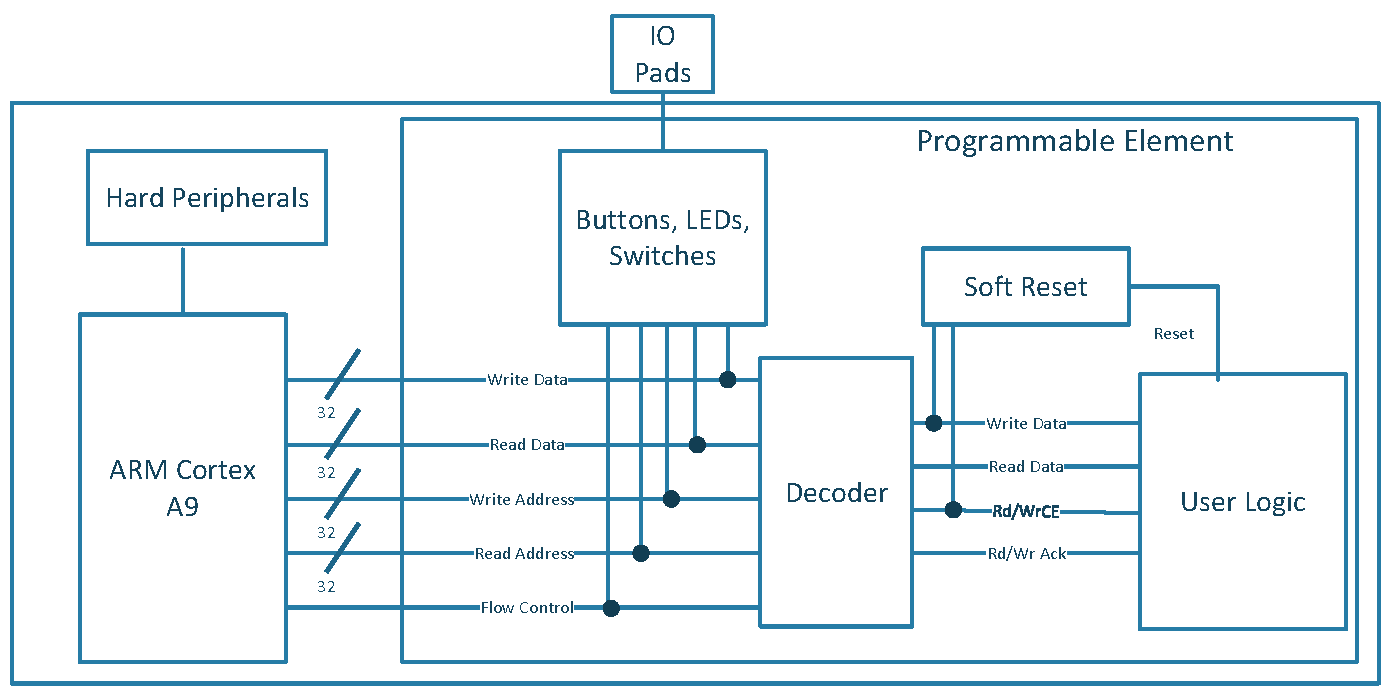
\includegraphics[scale=.35]{Images/coprocessor-template.pdf}
\caption{ Basic Coprocessor Template}
\label{fig:template}
\end{figure} 


\begin{figure}[!th]
\centering
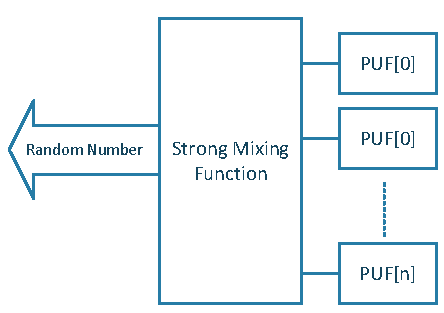
\includegraphics[scale=.75]{Images/trng.pdf}
\caption{PUF Array As TRNG }
\label{fig:trng}
\end{figure} 




\subsection{AXI Bus}

\subsection{TRNG Entropy Source}

The entropy source for the TRNG is based on a FPGA-based Physically Unclonable Function (PUF) design \cite{fpga_puf}. The PL of the Zynq 7000 is based on the Virtex-5 architecture, making porting the design a trivial affair. Given this,  the mechanics of the entropy source will only be summarized here. 

The entropy source consists of a large array of identical cells. Each cell is an FPGA-based analogue to an SRAM PUF. For example, in Fig.~\ref{conceptualdesign}, if both switches are initially closed, then the capacitors at Q1 and Q2 are both charged. Then at $t$=0, the switches are opened and the circuit resolves to a stable state which depends on the  delay through the inverter and interconnects, as well as the switching threshold of the logic. If route R1 has a shorter delay, it will remain at logical 1 and force Q2 to logical 0. If route R2 has a shorter delay, it will remain at logical 1 and force Q1 to logical 0. Thus Q1 and Q2 will always resolve to opposing values, but which has which value depends on the physical properties of the hardware.  The PUF design is shown in Fig.~\ref{logicaldesign}.  The switches are replaced by combinational logic implemented in LUTs.


\begin{figure}
 \centering
  \subfloat[Conceptual]{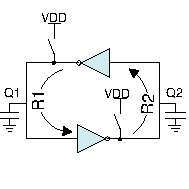
\includegraphics[scale=1]{Images/puf_concept.pdf}
				\label{conceptualdesign}}
 %  add desired spacing between images, e. g. ~, \quad, \qquad etc. (or a blank line to force the subfig onto a new line)
  \subfloat[Logical]{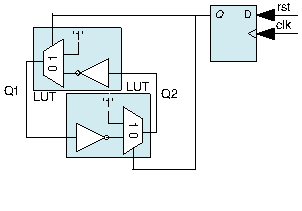
\includegraphics[scale=.9]{Images/puf_logical.pdf}
					\label{logicaldesign}}
   %add desired spacing between images, e. g. ~, \quad, \qquad etc. (or a blank line to force the subfig onto a new line)
  \caption{Selected PUF Design}
  \label{fig:design}
\vspace{-5mm}
\end{figure}

\subsection{Strong Mixing Function}

Because only a subset of PUF bits exhibit unstable behavior, a strong mixing function is needed to eliminate 0- or 1-bias, and to spread bit changes accross all output bits. For this project an opensource implementation of MD5 was used. It is designed for streaming operation and can complete one hash per AXI bus clock cycle, so that the average latency is eqivalent to a simple register file. It is the output of the mixing function which is considered the true-random number, and thus it is this value which is made available to the CPU over the AXI bus in the form of a memory-mapped register.  

\subsection{Software}

The software portion of our system consists of a simple testbench coupled with a small bare-metal support library. The example code below shows how registers 0 through 10 can be accessed as simple memory pointer dereferences, and Fig.~\ref{fig:dump} shows the results being printed over the serial port to a terminal. Note that \emph{u64} represents a 64-bit datatype. 

\begin{algorithm}
  \caption{Accessing Peripheral Registers}\label{euclid}
  \begin{algorithmic}[1]
    \Procedure{DumpRegs}{}
      \For{\texttt{i=0 to 10}}
	\State $offset\gets (i<<3)$
        \State $r\gets *( u64 *) (TRNG\_BASE\_ADDR+offset)$
      \EndFor
      \State \textbf{return} $b$
    \EndProcedure
  \end{algorithmic}
\end{algorithm}


\begin{figure}[!th]
\centering
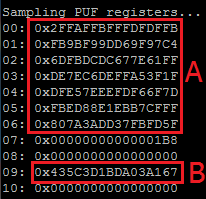
\includegraphics[scale=.9]{Images/dump2.png}
\caption{ Terminal Session Reading Out 64-bit TRNG register contents. (A) Raw PUF bits (debug only) (B) Hashed PUF bits}
\label{fig:dump}
\end{figure} 


\section{System Performance}

Performance was assessed as the rate at which new register values can be read over the AXI bus. This is a function of a number of factors:

\begin{enumerate}
  \item User Logic
  \begin{enumerate}
    \item Time to Assert RVALID
    \item Maximum clock rate which ensure timing closure
  \end{enumerate}
  \item Bus Interface Clock. Besides user logic, depends on: 
  \begin{enumerate}
    \item Address decoding logic (implemented in PL) 
   \item  Interconnect structure (presence of handshaking logic, bus width conversions, etc)
  \end{enumerate}
  \item Interconnect Structure 
 \begin{enumerate}
    \item Shared vs. Crossbar
    \item CPU port (GP vs HS)
    \item Bus width (eg. 32-bit vs 64 bit)
    \item Extra FIFOs, extra address or data registers (eg. to meet timing), etc
  \end{enumerate}
  \item CPU software
 \begin{enumerate}
    \item Compiler Optimization Level
    \item Transfer width (eg. 32-bit vs 64 bit) 
  \end{enumerate}
\end{enumerate}

Timing was assessed by performing 100,000 reads in a loop, using compiler optimization flag -O3, with an AXI bus frequency of 100Mhz. The difference  between the value in the Global Timer after the loop and before the loop can be used to derive the delay. The Global Timer is a hardware timer running at half the core CPU frequency so there is no extra overhead associated with it. Note that we did not explore the Streaming mode for AXI; this requires a significantly different approach which was not feasible in the project time frame. The benchmark data is shown below:

\begin{table}[h]
\begin{tabular}{@{}lll@{}}
\toprule
Setup                                 & Total Time (ms) & Transfer Rate (Mbps) \\ \midrule
AXI4-Lite (32-bit)                    & 13              & 246                             \\
AXI4 64-bit (1x 32-bit word transfer) & 15              & 213                             \\
AXI4 64-bit (2x 32-bit word transfer) & 18              & 355                             \\ \bottomrule
\end{tabular}
\end{table}

Although the time of a given read remains the same, as our user logic will always complete the RVALID handshake in 1 cycle, there is a measurable increase in latency between reads between AX4-lite and the full AXI4. We designed our peripheral to support 64-bit transfers to maximize throughput. However, since the basic memory-mapped peripheral is only attatched to the lower-performance CPU-AXI interface (GP0/GP1), which is 32-bits, the toolset will automatically insert bus resizing logic into the Programmable Logic which adds additional overhead. However, making full 64-bit transfers increases the overall throughput, in spite of the increase in latency. Performing a short "burst mode" transfer on the AXI4 bus saves cycles compared to making multiple separate transfers. 

\section{Conclusion}

In concluding, we were able to successfully meet our goals for the project, etc, etc.  



\bibliographystyle{IEEEtran}
\bibliography{main}

% that's all folks
\end{document}


